\section{Metodologie utilizzate}
Per il progetto didattico abbiamo deciso di utilizzare i seguenti approcci: l'algoritmo di \href{https://en.wikipedia.org/wiki/Logistic_regression}{\textit{Logistic Regression}} e le \href{https://en.wikipedia.org/wiki/Neural_network}{\textit{Neural Networks}}.\\
Tuttavia sono possibili altri approcci che, per rimanere all'interno dei tempi stabiliti, non siamo riusciti ad affrontare. 

\subsection{Reti neurali}
Il primo approccio che abbiamo scelto di utilizzare è stato quello delle reti neurali.
Per farlo ci siamo appoggiati alla libreria \href{https://www.tensorflow.org/}{\textit{TensorFlow}} la quale, dalla versione 2.0.0, integra \href{https://keras.io/}{\textit{Keras}} al suo interno.\\
Maggiori informazioni riguardanti l'integrazione di Keras sono presenti al seguente link \href{https://www.tensorflow.org/guide/keras}{\textit{tf.keras}}.\\ 
Questo permette di utilizzare TensorFlow come ecosistema e definisce la rete tramite delle classi messe a disposizione nelle API di Keras.\\
\subsubsection{Configurazione}
È stata scelto di utilizzare il tipo di rete \href{https://keras.io/getting-started/sequential-model-guide/}{\textit{Sequential}}, il problema infatti non prevedeva l'utilizzo di particolari tipi di layer.\\ 
In tal caso sarebbe stato oppurtuno utilizzare una rete di tipo \href{https://keras.io/getting-started/functional-api-guide/}{\textit{Functional}} che permette una maggiore libertà per la definizione della struttura della rete.
Tramite il metodo \textit{compile()} presente in Keras è possibile stabilire la:
\begin{enumerate}
\item \textbf{Loss functions}: \href{https://en.wikipedia.org/wiki/Cross_entropy}{\textit{binary crossentropy}} nel nostro caso, maggiori info al seguente link \href{https://keras.io/losses/}{\textit{loss functions}};
\item \textbf{Optimizer}: l'ottimizzatore che verrà utilizzato per l'aggiustamento dei pesi e per minimizzare la loss function.
Nel nostro caso \href{https://arxiv.org/pdf/1412.6980v8.pdf}{\textit{Adam}}. 
\item \textbf{Metrics}: la lista di metriche che verranno valutate dal modello durante la fase di training e testing.
Nel nostro caso è stata scelta la metrica di \href{https://keras.io/metrics/#binary_accuracy}{\textit{binart accuracy}}.  
\end{enumerate} 


\begin{figure}[H]
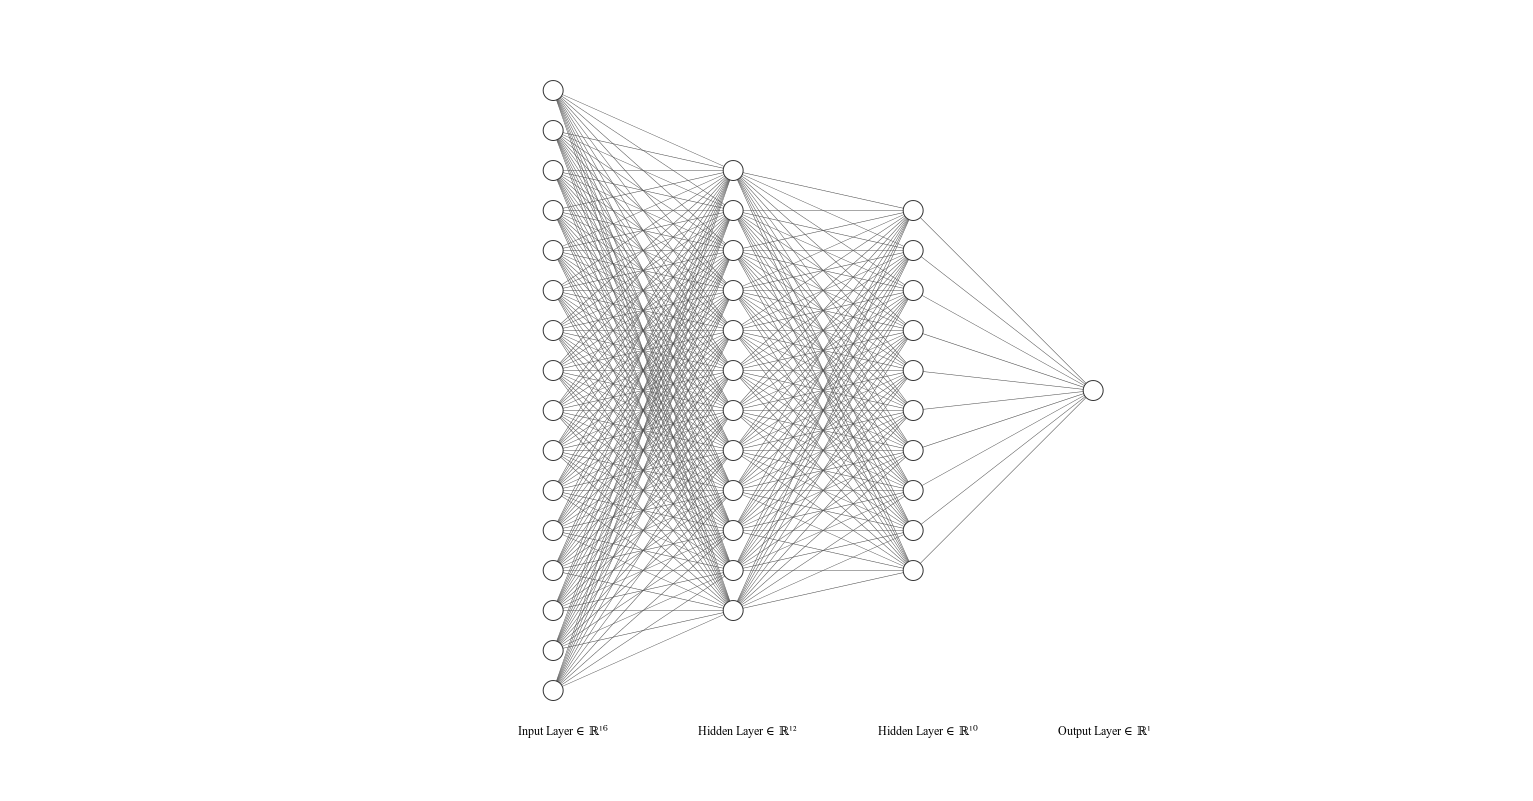
\includegraphics[scale=0.5,center]{img/nnExample.png}
\caption{Esempio di rete neurale}
\end{figure}

\subsection{Logistic Regression}